% XeLaTex
%\documentclass[review]{cvpr}
%\documentclass[final]{cvpr}
\documentclass[onecolumn]{article}
\usepackage[UTF8]{ctex}

%\usepackage{cvpr}
\usepackage{times}
\usepackage{epsfig}
\usepackage{graphicx}
\usepackage{amsmath}
\usepackage{amssymb}
\usepackage{subfigure}
\usepackage{overpic}

\usepackage{enumitem}
\setenumerate[1]{itemsep=0pt,partopsep=0pt,parsep=\parskip,topsep=5pt}
\setitemize[1]{itemsep=0pt,partopsep=0pt,parsep=\parskip,topsep=5pt}
\setdescription{itemsep=0pt,partopsep=0pt,parsep=\parskip,topsep=5pt}


\usepackage[pagebackref=true,breaklinks=true,colorlinks,bookmarks=false]{hyperref}

%\usepackage{multirow}
%\cvprfinalcopy % *** Uncomment this line for the final submission

\def\cvprPaperID{159} % *** Enter the CVPR Paper ID here
\def\confYear{CVPR 2020}
\def\httilde{\mbox{\tt\raisebox{-.5ex}{\symbol{126}}}}

\newcommand{\cmm}[1]{\textcolor[rgb]{0,0.6,0}{CMM: #1}}
\newcommand{\todo}[1]{{\textcolor{red}{\bf [#1]}}}
\newcommand{\alert}[1]{\textcolor[rgb]{.6,0,0}{#1}}

\newcommand{\IT}{IT\cite{98pami/Itti}}
\newcommand{\MZ}{MZ\cite{03ACMMM/Ma_Contrast-based}}
\newcommand{\GB}{GB\cite{conf/nips/HarelKP06}}
\newcommand{\SR}{SR\cite{07cvpr/hou_SpectralResidual}}
\newcommand{\FT}{FT\cite{09cvpr/Achanta_FTSaliency}}
\newcommand{\CA}{CA\cite{10cvpr/goferman_context}}
\newcommand{\LC}{LC\cite{06acmmm/ZhaiS_spatiotemporal}}
\newcommand{\AC}{AC\cite{08cvs/achanta_salient}}
\newcommand{\HC}{HC-maps }
\newcommand{\RC}{RC-maps }
\newcommand{\Lab}{$L^*a^*b^*$}
\newcommand{\mypara}[1]{\paragraph{#1.}}

\graphicspath{{figures/}}

% Pages are numbered in submission mode, and unnumbered in camera-ready
%\ifcvprfinal\pagestyle{empty}\fi
\setcounter{page}{1}

\begin{document}
% \begin{CJK*}{GBK}{song}

\renewcommand{\figref}[1]{图\ref{#1}}
\renewcommand{\tabref}[1]{表\ref{#1}}
\renewcommand{\equref}[1]{式\ref{#1}}
\renewcommand{\secref}[1]{第\ref{#1}节}
\def\abstract{\centerline{\large\bf 摘要} \vspace*{12pt} \it}

%%%%%%%%% TITLE

\title{第一次大作业\thanks{
本文为清华大学2022年春季学期数据安全课程作业}}

\author{xxx(2021xxx) \quad  
 \\
}

\maketitle
% \thispagestyle{empty}

%%%%%%%%% ABSTRACT
\begin{abstract}

摘要

\end{abstract}

%%%%%%%%% BODY TEXT %%%%%%%%%%%%%%%%%%%%%%%%%%%%%%%%%%%%%%%%
\section{第一节}\label{sec:sec:partone}

\section{第二节}\label{sec:parttwo}
SHA-3是第三代标准的哈希算法\cite{dworkin2015sha}\cite{paar2009understanding},

函数如式\ref{equ:sponge}:
\begin{equation}
\begin{array}{r}
\mathbf{SPONGE}[f,pad,r](N,d) 
\end{array}
 \label{equ:sponge}
\end{equation}
可用于将输入转为成指定长度的串,所以函数有两个参数:输入$N$和输出长度$d$。
\begin{figure}[h]
    \centering
    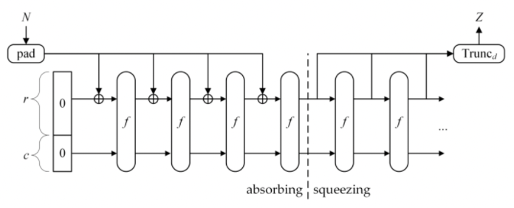
\includegraphics[width=\columnwidth]{figures/sponge.png}
    \caption{海绵结构示意图}
    \label{fig:sponge}
\end{figure}

 \begin{figure}[]
  \centering
  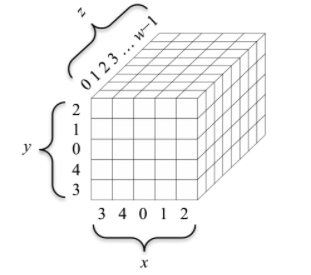
\includegraphics[width=6cm,height=5.8cm]{figures/xyz.png}
  \caption{状态数组结构示意图}
 \label{fig:xyz}
 \end{figure}




 

\section{彩虹表}\label{sec:partthree}

\section{结论}\label{sec:Conclusion}

本文


{
\bibliographystyle{ieee}
\bibliography{Saliency}
}


\paragraph{致谢.} 非常感谢老师xxx!也非常感谢我们助教老师的辛苦付出!



% \end{CJK*}
\end{document}
